\documentclass[11pt,letterpaper]{article}
% isms-27000-style.tex
% Suite preamble for the ISO/IEC 27000/27001/27002 ISMS engineering suite.
%
% RECONSTRUCTION PROVENANCE: the ten uploaded suite documents load a shared
% preamble with `\input{style.tex}`, but no `style.tex` was present in the
% upload batches or anywhere in this repository's history. This file is a
% documented, suite-specific reconstruction inferred from the macros, colors
% and environments the documents actually use (colors navy/teal/graytext/pale;
% tag commands \SourceTag, \EngineeringTag, \SourceNote{..}; breakable
% tcolorbox callouts; color-striped longtables; TikZ flow diagrams). It is
% NOT the recovered original style; the original visual design is unknown.
%
% pdfLaTeX only.
\usepackage[T1]{fontenc}
\usepackage[utf8]{inputenc}
\usepackage{lmodern}
\usepackage{microtype}
\usepackage[letterpaper,margin=0.9in,headheight=15pt]{geometry}
\usepackage[table]{xcolor}
\definecolor{navy}{HTML}{14355A}
\definecolor{teal}{HTML}{0A7580}
\definecolor{graytext}{HTML}{55616E}
\definecolor{pale}{HTML}{EFF5F7}
\usepackage{amsmath,amssymb}
\usepackage{array,booktabs,longtable,tabularx,multirow}
\usepackage{enumitem}
\usepackage[most]{tcolorbox}
\usepackage{tikz}
\usetikzlibrary{arrows.meta,positioning,shapes.geometric,fit,calc}
\usepackage{needspace}
\usepackage{titlesec}
\usepackage{fancyhdr}
\usepackage{lastpage}
\usepackage{hyperref}
\hypersetup{colorlinks=true,linkcolor=navy,urlcolor=teal,citecolor=navy,pdfauthor={ISMS Engineering Documentation Suite},pdfsubject={Original supporting guidance for ISO/IEC 27000, 27001 and 27002}}
\setlength{\parindent}{0pt}
\setlength{\parskip}{5pt plus 1pt}
\setlength{\emergencystretch}{2em}
\renewcommand{\arraystretch}{1.18}
\setlist[itemize]{itemsep=2pt,topsep=3pt,leftmargin=1.5em}
\setlist[enumerate]{itemsep=2pt,topsep=3pt,leftmargin=1.7em}
\titleformat{\section}{\Large\bfseries\color{navy}}{\thesection}{0.7em}{}[\vspace{-3pt}\color{teal}\titlerule]
\titleformat{\subsection}{\large\bfseries\color{navy}}{\thesubsection}{0.6em}{}
\titleformat{\subsubsection}{\normalsize\bfseries\color{teal}}{\thesubsubsection}{0.55em}{}
\pagestyle{fancy}
\fancyhf{}
\fancyhead[L]{\sffamily\footnotesize ISO/IEC 27000 series | ISMS Engineering}
\fancyhead[R]{\sffamily\footnotesize\color{graytext} Independent companion}
\fancyfoot[L]{\sffamily\scriptsize Original explanatory material; consult the licensed standards}
\fancyfoot[R]{\sffamily\scriptsize\thepage\ / \pageref{LastPage}}
\renewcommand{\headrulewidth}{0.3pt}
% Inline provenance tags used throughout the suite: \SourceTag marks
% statements grounded in the standards; \EngineeringTag marks original
% engineering interpretation. Both are zero-argument label commands.
\newcommand{\SourceTag}{\textsf{\footnotesize\bfseries\color{navy}[Standard]}~}
\newcommand{\EngineeringTag}{\textsf{\footnotesize\bfseries\color{teal}[Engineering]}~}
\newcommand{\SourceNote}[1]{\par\smallskip{\footnotesize\color{graytext}\textit{Trace: #1.}}\par}

\begin{document}
\pagenumbering{roman}
\begin{titlepage}
\vspace*{1.2in}
{\color{teal}\rule{\textwidth}{4pt}}\par\vspace{20pt}
{\Huge\bfseries\color{navy} ISMS Foundations and Vocabulary}\par\vspace{18pt}
{\Large\color{graytext} Concepts, terminology, process model and interpretation rules}\par\vspace{1.3in}
{\large ISO/IEC 27000:2018 $\vert$ ISO/IEC 27001:2022 $\vert$ ISO/IEC 27002:2022}\par
\vfill
\textbf{Independent educational and engineering implementation reference}\par
Version 1.0 $\cdot$ October 2026\par
{\small Original explanatory material. Source standards are copyrighted; consult licensed originals for authoritative requirements.}\par
\end{titlepage}
\tableofcontents\clearpage\pagenumbering{arabic}
\begin{tcolorbox}[title={How to use this reference},colback=pale,colframe=teal,breakable]
\SourceTag ISO/IEC 27000:2018 supplies overarching ISMS concepts and common terms. ISO/IEC 27001:2022 refers to ISO/IEC 27000 for terminology. \EngineeringTag This document connects that vocabulary to concrete workflows and avoids assigning a certification requirement to a vocabulary statement.
\end{tcolorbox}
\section{Standards relationship}
\small\rowcolors{2}{pale}{white}\begin{longtable}{p{.24\linewidth}p{.23\linewidth}p{.47\linewidth}}
\rowcolor{navy} \textcolor{white}{\textbf{Document}} & \textcolor{white}{\textbf{Principal role}} & \textcolor{white}{\textbf{How this suite uses it}}\\
\endfirsthead
\rowcolor{navy} \textcolor{white}{\textbf{Document}} & \textcolor{white}{\textbf{Principal role}} & \textcolor{white}{\textbf{How this suite uses it}}\\
\endhead
ISO/IEC 27000:2018 & Overview and vocabulary & Conceptual model and consistent terminology\\
ISO/IEC 27001:2022 & ISMS requirements & Clauses 4--10, risk treatment, SoA and audit basis\\
ISO/IEC 27002:2022 & Information security control guidance & Controls 5.1--8.34, recommended implementation approaches\\
\end{longtable}\normalsize

\section{ISMS as a management system}
\SourceTag The ISMS preserves confidentiality, integrity and availability by governing security risks in the context of organizational objectives. Its effectiveness depends on integrating policy, leadership, roles, processes and improvement rather than merely deploying tools.

\EngineeringTag Model the ISMS as a persistent graph: \texttt{stakeholder} $\rightarrow$ \texttt{obligation} $\rightarrow$ \texttt{objective} $\rightarrow$ \texttt{risk} $\rightarrow$ \texttt{treatment}. The assurance chain continues as \texttt{control} $\rightarrow$ \texttt{evidence} $\rightarrow$ \texttt{assessment} $\rightarrow$ \texttt{improvement}. Every edge should be attributable to an owner and a decision date.
\begin{center}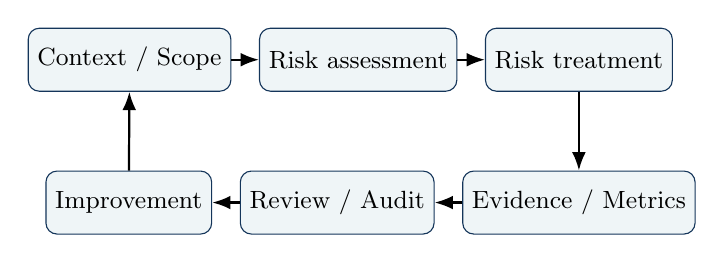
\begin{tikzpicture}[node distance=.35cm, every node/.style={font=\small},b/.style={draw=navy,fill=pale,rounded corners,align=center,minimum height=.8cm,minimum width=2.1cm},>=Latex]
\node[b](c){Context / Scope};\node[b,right=of c](r){Risk assessment};\node[b,right=of r](t){Risk treatment};
\node[b,below=1cm of t](e){Evidence / Metrics};\node[b,left=of e](a){Review / Audit};\node[b,left=of a](i){Improvement};
\draw[->,thick] (c)--(r);\draw[->,thick](r)--(t);\draw[->,thick](t)--(e);\draw[->,thick](e)--(a);\draw[->,thick](a)--(i);\draw[->,thick](i)--(c);
\end{tikzpicture}\end{center}
\section{Operational glossary (paraphrased concepts)}
\small\rowcolors{2}{pale}{white}\begin{longtable}{p{.25\linewidth}p{.69\linewidth}}
\rowcolor{navy} \textcolor{white}{\textbf{Term}} & \textcolor{white}{\textbf{Engineering interpretation and use}}\\
\endfirsthead
\rowcolor{navy} \textcolor{white}{\textbf{Term}} & \textcolor{white}{\textbf{Engineering interpretation and use}}\\
\endhead
Asset & Something of value to the organization; record information and supporting resources without equating every asset with an IT device.\\
Confidentiality & Prevention of disclosure to parties without authorization; test through access boundaries and data movement.\\
Integrity & Accuracy and completeness of information; assess integrity in processes, storage and transfers.\\
Availability & Usability when an authorized party needs information; link to continuity objectives and dependency failure.\\
Information security & Protection of confidentiality, integrity and availability; other trust properties may also matter.\\
ISMS & Interacting policies, objectives, accountabilities, procedures and controls for governing information security.\\
Management system & Coordinated organizational elements that establish direction and achieve measurable objectives.\\
Policy & Top-management direction expressed formally; distinguish from procedural work instructions.\\
Objective & An intended result, which should have accountable evaluation and a target if practicable.\\
Interested party & An organization/person with relevance to decisions or affected outcomes; may impose requirements.\\
Scope & Business/technical boundaries and dependencies for the ISMS, documented for review.\\
Risk & Effect of uncertainty on objectives; formulate as a credible scenario, not simply a scanner finding.\\
Risk source & Element with potential to produce risk; record actors, dependencies and hazardous conditions.\\
Likelihood & Chance of a risk scenario materializing; define the measurement basis.\\
Consequence & Outcome affecting objectives; assess CIA impact and downstream operational effects.\\
Level of risk & Combination of likelihood and consequence under an established scoring method.\\
Risk assessment & Structured identification, analysis and evaluation of information security risks.\\
Risk treatment & Choice and execution of responses that adjust or handle risk.\\
Residual risk & Risk remaining after treatment; not automatically acceptable.\\
Risk owner & Accountable business decision-maker for a defined risk and remaining exposure.\\
Control & ISO/IEC 27000:2018 describes a risk-modifying measure; ISO/IEC 27002:2022 additionally uses maintaining and/or modifying risk. Include management and technical measures.\\
Control objective & The outcome intended from control activity; assess it with evidence, not merely policy presence.\\
Effectiveness & Extent to which planned work and intended results are actually achieved.\\
Performance & Measurable outcome; distinguish an operational result from an implementation checkbox.\\
Monitoring & Determining current state; does not alone prove corrective action.\\
Measure & Value assigned through a measurement method.\\
Audit & Independent, documented and objective evaluation against specified criteria.\\
Audit evidence & Verifiable records, observations and other material used in an audit.\\
Nonconformity & Failure to fulfill a relevant requirement; document clause and evidence.\\
Correction & Immediate action addressing an observed nonconformity.\\
Corrective action & Action addressing a cause to prevent recurrence, including an effectiveness check.\\
Continual improvement & Recurring efforts that enhance ISMS performance over time.\\
Documented information & Controlled information and records needed to operate or demonstrate the ISMS.\\
Governance of information security & How information security activities are directed and controlled.\\
Information security event & Observed circumstances that may indicate security-control failure or security concern.\\
Information security incident & Related events capable of harming assets or operations; keep triage decisions documented.\\
\end{longtable}\normalsize

\section{Terminology crosswalk: event, incident, and nonconformity}
\begin{itemize}
\item An \textbf{event} is an observation; an \textbf{incident} results from assessment of potentially harmful related events. A false alert may be an event without being an incident.
\item A \textbf{nonconformity} is a failure against an ISMS requirement, which can exist independently of a cyber incident. For example, an unapproved policy version may require corrective action without data compromise.
\item A \textbf{risk} remains prospective: it can exist without an event, incident or nonconformity. Keep separately linked records.
\end{itemize}

\section{Worked example: source-code access}
A third-party contractor receives permanent write access to a production repository. \textbf{Asset:} business application source code. \textbf{Scenario:} unauthorized alteration of a release. \textbf{Treatment:} managed identities, least privilege, protected branches and review. \textbf{Candidate controls:} 5.15, 5.18, 8.2, 8.4, 8.25 and 8.32. \textbf{Evidence:} repository access review, pull-request approvals and audit events. \textbf{Test:} attempt a disallowed direct push with a restricted test identity. \textbf{Risk ownership:} accountable application/product owner.
\section{Interpretation safeguards}
\begin{itemize}
\item Use the supplied 2018 and 2022 editions when interpreting terms; record edition-specific differences rather than silently replacing them.
\item Keep original control IDs and clause references as pointers to the licensed standard; this suite does not reproduce the normative wording.
\item Do not infer that every Annex A control is required in every organization: apply risk treatment, check Annex A for omissions and justify exclusions.
\item Use authoritative text and external certification rules for formal audit findings and claims of conformity.
\end{itemize}

\clearpage\section*{Source and interpretation policy}
\addcontentsline{toc}{section}{Source and interpretation policy}
\textbf{Source editions:} ISO/IEC 27000:2018 (overview and vocabulary); ISO/IEC 27001:2022 (requirements and normative Annex A); ISO/IEC 27002:2022 corrected 2022-03 (control guidance). Specific clause identifiers are references to the supplied editions, not reproduced control text.\par
\textbf{Interpretation:} ``Source-grounded paraphrase'' describes a concept in the cited source. ``Engineering recommendation'' is a practical model, technology choice, owner, evidence example, frequency, template or scoring convention authored for this suite; it is not a claim that ISO prescribes that exact approach.\par
\textbf{Conformity:} Clauses 4--10 of ISO/IEC 27001 govern ISMS conformity. Applicability of controls is determined through risk treatment, with Annex A used as a completeness cross-check and exclusions justified in the Statement of Applicability (SoA). Source documents alone neither certify an ISMS nor prove control operating effectiveness.\par
\textbf{Source licensing:} Do not distribute or embed the licensed standard PDFs in repositories or distribute copied normative text. Review the editions, amendments, and certification scheme applicable to each assessment before relying on this work.\par
\end{document}
